% --------------------------------------------------------------------------
% Шаблон презентации в стилистике Университета ИТМО
% Версия шаблона 2.1. Также шаблон доступен на сайтах:
% https://www.overleaf.com/read/rpkkfchcnbsc
% https://www.overleaf.com/latex/templates/itmo-beamer-theme/fpttrgnmqwsb
% https://github.com/AlexZabashta/ITMO-Beamer-theme
% --------------------------------------------------------------------------

% Внимание!!!
% Этот документ создан для примера использования beamer стиливика.
% Не стоит воспринимать его как урок Latex или beamer!
% Ознакомьтесь с возможностями Latex и beamer (хотя бы базовыми) отдельно.


\documentclass[aspectratio=169]{beamer}
\usepackage{ITMOtheme}


% Без этой команды он иногда ругается.
\hypersetup{unicode=true}

% Пакет для "русификации" Latex.
\usepackage[english,russian]{babel}

% Чтобы адекватно работало копирование текста из полученной .pdf-ки.
\usepackage{cmap}


% Это нужно, чтобы он называл рисунки без сокращения "рис.".
% Таблицы он называет без сокращения по умолчанию.
\addto\captionsrussian{\renewcommand{\figurename}{Рисунок}}

% Пакет для использования запятой в качестве десятичного разделителя.
% Следите, чтобы в формулах запятые стояли с пробелами, там где они запятые. Например $v = (x, y, z)$
\usepackage{icomma}

% Это единственный пакет для библиографии, который у меня заработал с \footcite шаблоном.
% В презентациях лучше делать её руками через \footnote!
% \usepackage[style=mla]{biblatex}
% \addbibresource{references.bib}


% Рисунок для титульного слайда.
\titlegraphic{
\includegraphics[scale=.8]{itmo/logo_rus_vert_blue.pdf}}


% Поля title, author, subject, keywords используются при формировании pdf документа.
% Поэтому их нужно заполнять, даже если вы формируете титульный слайд руками.

% Формат: \title[Короткое название]{Полное название}
\title[ITMO LaTex]{Приложение MEET ME}

%\subtitle[short subtitle]{long subtitle}

% В квадратных скобках короткая запись авторов.
\author[Шишминцев Д. В.]{Шишминцев Дмитрий Владимирович}

%\institute[short institute name]{long institute name}

\where{Санкт-Петербург}
\date{\today}

% Тематика и ключевые слова.
\subject{Beamer template}
\keywords{ITMO University, LaTex teamplate, beamer}


% По умолчанию внизу каждого слайда пишется название презентации (\inserttitle).
% Этот текст можно заменить на другой, например:
\setfootlinetext{\insertsection}


\begin{document}

% [plain] - модификатор для создания пустого слайда (без нижней полосы).
% Идеально подходит для создания первого (титульного) и последнего слайда с полигональным фоном,
% либо для переходных слайдов между главами или слайдов с оглавлением.

% \titlepage - команда для автоматической генерации контента титульного слайда.
\begin{frame}[plain]
    \titlepage
\end{frame}

% \itmopolygons - команда для создания полигонального фона.
% Используется для создания фона на первом (титульном) и последнем слайде.


% Если вас не устраивает контент стандартного титульного слайда,
% то можете сами его скомпоновать, либо исправить .sty файл.


\begin{frame}{Содержание}
    \tableofcontents
\end{frame}


% Не стоит делать оглавление в коротких презентациях.
% Переходы между главами лучше делать "руками".



\section{Введение}

\begin{frame}
\frametitle{Введение}
Данная презентация содержит в себе основную идею будущей информационной системы с рабочим названием MEET ME, планируемый набор ее функций, основных пользователей этой информациионной системы, прототип интерфейса, а так же анализ рынка.

\end{frame}


\section{Описание идеи информационной системы}

\subsection{Идея}
\begin{frame}
\frametitle{Идея}
\begin{itemize}
    \item Веб-приложение для планирования встреч с друзьями в виде календаря. 
    \item Приложение показывает пользователям пересечения свободного времени с их друзьями или группами друзей.
    \item Приложение имеет только прямых конечных пользователей.
    \item С помощью приложения пользователи смогут эффективно планировать встречи с друзьями.
    \item Приложение ориентировано на широкий круг людей.
\end{itemize}
    
\end{frame}

\subsection{Функционал}
\begin{frame}
\frametitle{Функционал}
\begin{columns}[c] 

    \column{.45\textwidth}{
        
        \begin{itemize}
            \item Регистрация аккаунта;
            \item Настройка свободного времени вручную;
            \item Настройка свободного времени основываясь на рекомендациях данных системой благодаря импорту расписания из Google Calendar / .cal файлов;
            \item Редактирование свободного времени;
        \end{itemize}
    }
    
    \column{.45\textwidth}{
        \begin{itemize}
            \item Отправка и принятие заявок в друзья;
            \item Создание группы из существующих друзей;
            \item Отправка приглашений на встречу;
            \item Принятие/Отклонение встречи;
            \item Утверждение групповой встречи методом голосования.
        \end{itemize}
    }
    
    \end{columns}
\end{frame}

\subsection{Прототип}

\begin{frame}
\begin{figure}
    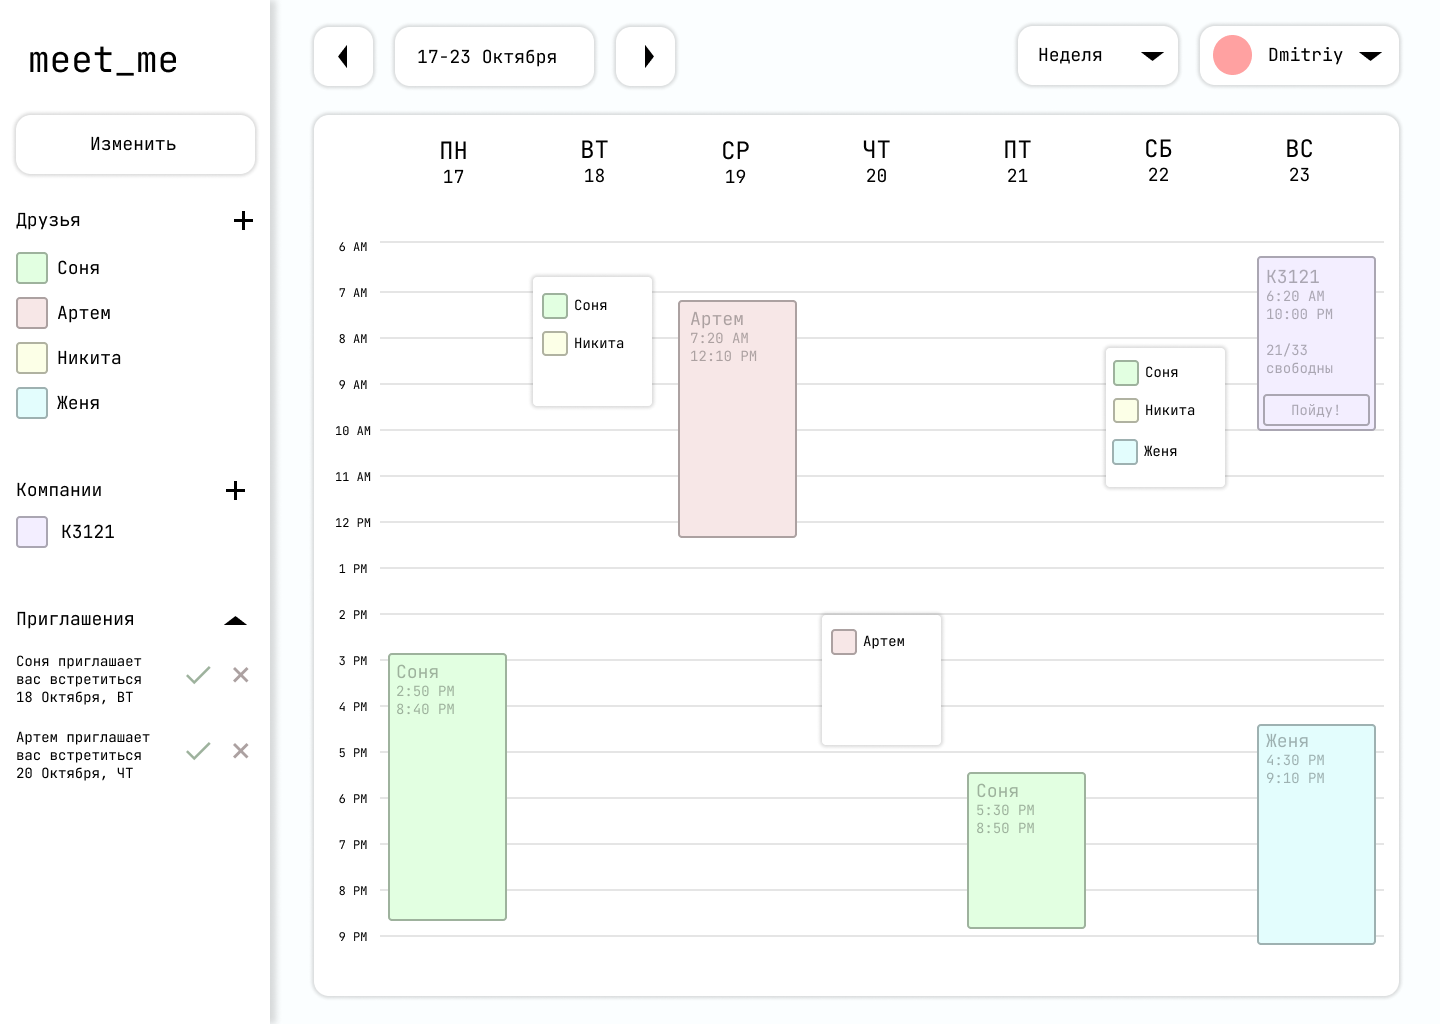
\includegraphics[scale=.2]{img/prototype.png}
    \caption{Прототип интерфейса}
\end{figure}
\end{frame}


\section{Анализ рынка}

\subsection{Сравнение с аналогами}
\begin{frame}
    \frametitle{Сравнение с аналогами}
    
    % Лучше не использовать table в презентациях, только tabular. А описание таблиц делать руками.
    
    \begin{table} 
    \begin{tabular}{r | r r r r r} 
              & MEET ME &  NeedToMeet &  Rally & WhenAvalible \\ \hline
             Настройка расписания    & Да  & Да  & Нет & Да \\
             Импорт расписания       & Да  & Нет & Нет & Да \\
             Список друзей           & Да  & Да  & Нет & Нет \\
             Личные встречи          & Да  & Да  & Да  & Да \\
             Групповые встречи       & Да  & Да  & Да  & Да \\
             Отправка приглашений    & Да  & Да  & Нет & Да \\
             Создание опросов        & Нет & Да  & Да  & Да \\
             Пересечения & Да  & Нет & Нет & Нет \\
             Календарный вид         & Да  & Да  & Нет & Нет \\
             Стоимость               & Бесплатно & 19\$/год & Бесплатно & 38\$/год \\
    \end{tabular} 
    \end{table}
    \end{frame}

\subsection{Обоснование необходимости разработки}
\begin{frame}
\frametitle{Обоснование необходимости разработки}

\begin{itemize}
    \item Идея уникальна 
    \item Сервисы имеющие похожий функционал завязаны на одном пользователе.
    \item Приложение заинтересует широкий круг людей
    \item Более удобный инструмент для планирования
\end{itemize}
\end{frame}

\section{Заключение}

\begin{frame}
    \frametitle{Заключение}
    Описан основной функционал системы, основные пользователи, создан прототип интерфейса, а так же был проведен анализ рынка и
    приведено описание аналогов.
\end{frame}

\begin{frame}[plain]
    \itmopolygons{
        \vfill
        \Huge{Спасибо за внимание!}
        \vfill
        
\includegraphics[scale=.5]{itmo/slogan.pdf}
    }
\end{frame}

\end{document}
